\documentclass[12pt,a4paper]{article}
\usepackage[margin=2.0cm]{geometry}
\usepackage[T1]{fontenc}
\usepackage{lmodern}
\usepackage{enumitem}
\usepackage{xcolor}
\usepackage{booktabs}
\usepackage{tabularx}
\usepackage{array}
\usepackage{graphicx}
\usepackage{float}
\usepackage{tikz}
\usetikzlibrary{arrows.meta,positioning,fit,backgrounds,calc}
\usepackage{caption}
\usepackage[hidelinks]{hyperref}
\usepackage{xurl}
\usepackage{titlesec}

\definecolor{head}{RGB}{25,60,120}
\titleformat{\section}{\Large\bfseries\color{head}}{\thesection.}{0.6em}{}
\titleformat{\subsection}{\large\bfseries\color{head}}{\thesubsection}{0.6em}{}
\setlist{itemsep=3pt,topsep=4pt,leftmargin=1.5em}
\setlength{\parindent}{0pt}
\setlength{\parskip}{6pt}
\linespread{1.05}
\renewcommand{\arraystretch}{1.25}
\newcolumntype{L}{>{\raggedright\arraybackslash}X}
\newcolumntype{C}{>{\centering\arraybackslash}X}
\graphicspath{{figures/}}

\tikzset{
  box/.style={draw, rounded corners=3pt, align=center, minimum height=1.0cm, text width=2.6cm, font=\small, fill=#1},
  box/.default={white},
  arr/.style={-{Stealth[length=2.5mm]}, thick},
  darr/.style={{Stealth[length=2.5mm]}-{Stealth[length=2.5mm]}, thick},
  layer/.style={draw, dashed, rounded corners=6pt, inner sep=8pt}
}

\begin{document}

%================ TITLE PAGE ================
\begin{titlepage}
\centering
\vspace*{1.5cm}
{\large IT457 -- Cloud Computing\par}
\vspace{0.3cm}
{\large Case Study Project: Final Report\par}
\vspace{1.8cm}
{\Huge\bfseries\color{head} GE Predix\par}
\vspace{0.4cm}
{\LARGE Industrial IoT Cloud Platform and\\[4pt] GE's Migration to the Cloud\par}
\vspace{1.2cm}
{\Large Hands-on exercise: \textbf{Mini-Predix}\\[4pt]
\large migrated from Docker to VPS servers and AWS (EC2 + RDS),\\ with performance, cost and scaling analysis\par}
\vspace{2cm}
{\large\bfseries Group 27\par}
\vspace{0.3cm}
{\large Theme: Migration \& Transformation\par}
\vspace{0.8cm}
\begin{tabular}{ll}
\toprule
\textbf{Student ID} & \textbf{Name} \\
\midrule
202303009 & Nidhi Dodiya \\
202303046 & Param Savjani \\
202301436 & Vraj Makmana \\
\bottomrule
\end{tabular}
\vfill
{\large Code: \url{https://github.com/paramsavjani/it457-mini-predix}\par}
\vspace{0.3cm}
{\large October 2026\par}
\end{titlepage}

\setcounter{tocdepth}{1}
\tableofcontents
\newpage

%================ 1 INTRODUCTION ================
\section{Introduction}
General Electric (GE) builds jet engines, gas turbines, locomotives and medical equipment. Around 2013
it set out to become a ``digital industrial'' company, which produced two cloud stories:
\begin{enumerate}
  \item \textbf{Predix}, a cloud platform built by GE for the \emph{Industrial Internet of Things (IIoT)}:
        collect data from machines, analyse it and predict failures before they happen [1,2].
  \item \textbf{GE's own IT migration}, moving thousands of internal applications out of its data
        centers and onto Amazon Web Services (AWS) [4,5].
\end{enumerate}

This report has two parts.

\textbf{Part A (Sections 2--6)} studies the case: the problem GE faced, the Predix architecture, the
cost and business outcome, and the lessons for cloud computing.

\textbf{Part B (Sections 7--14)} describes our hands-on exercise. We built \textbf{Mini-Predix}, a small
industrial IoT monitoring application that copies Predix's core idea, and migrated it the way GE
migrated its IT: from a local Docker setup (``on-premises''), to rented virtual machines
(lift-and-shift), to a managed cloud database (refactor). We ran it on five deployments in three
locations, load-tested each one, and compared performance, monthly cost, operations effort and how
each option scales. Every number in Part B was measured by us; the raw data is in the GitHub
repository.

%================ PART A: GE CASE (from the Week 2 report) ================
\section{Background}
\subsection{GE and the Industrial Internet}
GE's machines operate in some of the most critical environments in the world: power plants, aircraft, railways and
hospitals. Each machine is fitted with many sensors. A single gas turbine or jet engine can produce large volumes of
data every hour of operation. Historically, this data was used only locally, for real-time control, and then mostly
discarded.

GE coined the term \emph{Industrial Internet} for the idea of connecting these machines to the network, collecting
their data centrally, and applying analytics to improve efficiency. Even small improvements matter at this scale:
a 1\% fuel saving across an airline fleet or a power grid is worth a very large amount of money.

\subsection{Timeline}
\begin{center}
\begin{tabularx}{\linewidth}{@{}p{2.2cm}L@{}}
\toprule
\textbf{Year} & \textbf{Event} \\
\midrule
2013 & GE launches Predix as its software platform for the Industrial Internet of Things [3,9]. \\
2013 & GE invests \$105 million in Pivotal, the company that led the Cloud Foundry project [3]. \\
2015 & GE Digital is formed. In August, GE announces \textbf{Predix Cloud}, a PaaS for industrial data [1]. \\
2015 & At AWS re:Invent, GE's CIO presents the plan to move 9,000 workloads to AWS and shrink from 34 data centers to 4 [4]. \\
2016 & Predix Cloud becomes commercially available to external customers [3]. \\
2017 & GE names AWS its \emph{preferred cloud provider}; over 2,000 applications already migrated [5]. \\
2017 & Reports of technical problems; Predix takes a ``time out'' from the market [7]. \\
2018 & New leadership refocuses GE Digital on Power, Aviation and Healthcare and cuts costs [8]. \\
Dec 2018 & GE announces plans for a separate industrial IoT software company with \$1.2B revenue [9]. \\
Oct 2019 & GE decides to keep GE Digital inside the company, with a narrower vertical focus [9]. \\
\bottomrule
\end{tabularx}
\end{center}

%================ 3 PROBLEM ================
\section{Problem Statement}
GE faced two separate but related problems: one on the product side and one on the internal IT side.

\subsection{Problem 1: Unused industrial data}
\begin{itemize}
  \item \textbf{Volume and velocity:} industrial machines generate continuous, high-frequency time-series data. Traditional
        enterprise databases and on-premises servers were not designed for this load.
  \item \textbf{Unplanned downtime is expensive:} when a turbine or engine fails without warning, the cost includes
        repairs, lost production and safety risk. Customers wanted \emph{predictive maintenance}, meaning that
        the machine's data should warn them before a failure happens.
  \item \textbf{Remote and unreliable connectivity:} machines are often located at remote sites such as oil rigs, wind farms or
        aircraft, where network connections are slow or intermittent.
  \item \textbf{Security and reliability:} the data comes from critical infrastructure, so the platform must be highly
        secure and always available.
  \item \textbf{Generic clouds lacked industrial features:} in 2015, general public clouds did not offer ready-made
        services for industrial protocols, asset models or physics-based analytics.
\end{itemize}

\subsection{Problem 2: Expensive, fragmented internal IT}
\begin{itemize}
  \item GE had grown through decades of acquisitions, leaving it with a very large and fragmented IT estate: around
        \textbf{9,000 workloads spread across 34 data centers} in 2015 [4].
  \item Running so many data centers meant high fixed costs for hardware, power, cooling, staff and maintenance.
  \item Provisioning new servers was slow, which slowed down development teams.
  \item Many duplicated systems existed across business units, making the estate hard to manage and secure.
\end{itemize}

\subsection{Why the cloud?}
Both problems point to the same core benefits of cloud computing: \emph{elastic} storage and compute that can grow with
data volume, \emph{pay-as-you-go} pricing instead of large up-front investment, \emph{managed services} that remove
operational work, and \emph{global reach} for customers and machines located around the world.

%================ 4 SOLUTION ================
\section{Solution and Architecture}
\subsection{Predix platform overview}
Predix was designed as a \textbf{Platform-as-a-Service (PaaS)} for industrial applications. Its architecture has three
main tiers: the \emph{edge}, the \emph{cloud platform}, and the \emph{applications} built on top [1,6].

\begin{figure}[h]
\centering
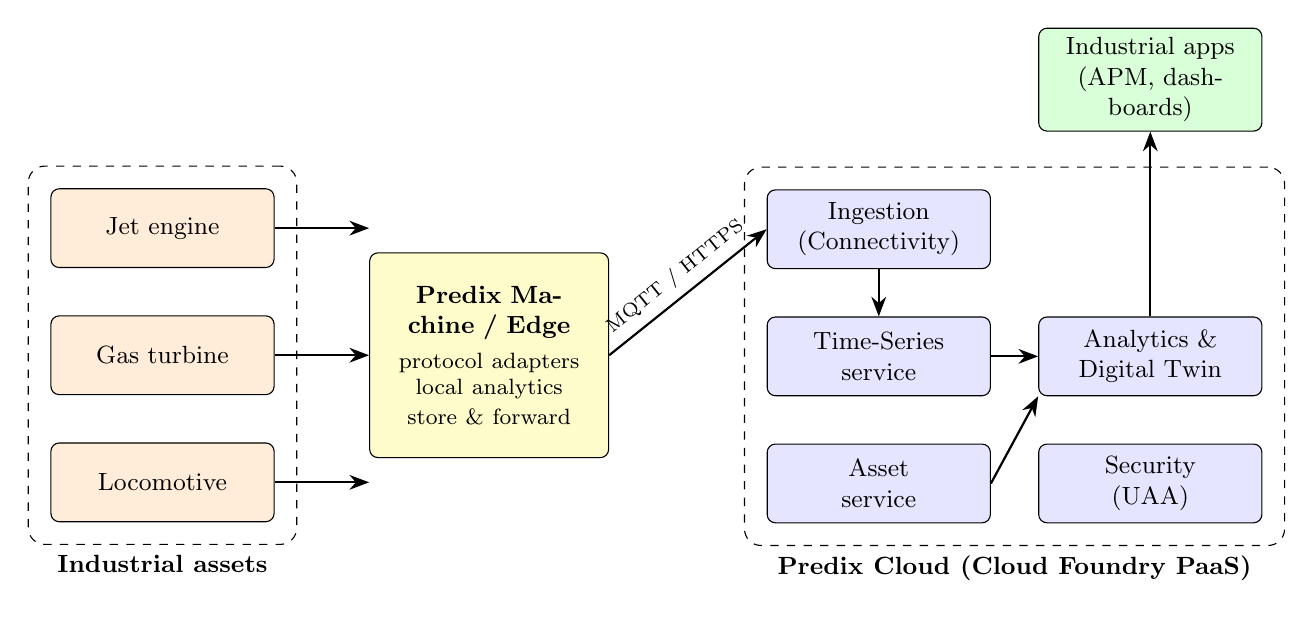
\begin{tikzpicture}[node distance=0.6cm and 0.6cm]
  % Assets
  \node[box=orange!15] (a1) {Jet engine};
  \node[box=orange!15, below=of a1] (a2) {Gas turbine};
  \node[box=orange!15, below=of a2] (a3) {Locomotive};
  % Edge
  \node[box=yellow!20, right=1.2cm of a2, text width=2.8cm, minimum height=2.6cm] (edge)
       {\textbf{Predix Machine / Edge}\\[3pt]\footnotesize protocol adapters\\ local analytics\\ store \& forward};
  % Cloud
  \node[box=blue!10, right=2.0cm of edge, yshift=1.6cm] (ingest) {Ingestion\\(Connectivity)};
  \node[box=blue!10, below=of ingest] (ts) {Time-Series\\service};
  \node[box=blue!10, below=of ts] (asset) {Asset\\service};
  \node[box=blue!10, right=0.6cm of ts] (analytics) {Analytics \&\\Digital Twin};
  \node[box=blue!10, below=of analytics] (sec) {Security\\(UAA)};
  % Apps
  \node[box=green!15] (apps) at ([yshift=1.9cm]analytics |- ingest) {Industrial apps\\(APM, dashboards)};
  % arrows
  \draw[arr] (a1.east) -- (edge.west |- a1.east);
  \draw[arr] (a2.east) -- (edge.west);
  \draw[arr] (a3.east) -- (edge.west |- a3.east);
  \draw[arr] (edge.east) -- node[midway, above, sloped, font=\scriptsize]{MQTT / HTTPS} (ingest.west);
  \draw[arr] (ingest) -- (ts);
  \draw[arr] (ts) -- (analytics);
  \draw[arr] (asset.east) -- (analytics.south west);
  \draw[arr] (analytics) -- (apps);
  % layers
  \begin{scope}[on background layer]
    \node[layer, fit=(ingest)(asset)(analytics)(sec), label={[font=\small\bfseries]below:Predix Cloud (Cloud Foundry PaaS)}] {};
    \node[layer, fit=(a1)(a3), label={[font=\small\bfseries]below:Industrial assets}] {};
  \end{scope}
\end{tikzpicture}
\caption{Simplified Predix architecture: assets $\rightarrow$ edge $\rightarrow$ cloud services $\rightarrow$ applications.}
\end{figure}

\subsection{Edge tier: Predix Machine}
Predix Machine (later Predix Edge) is software that runs on a gateway next to the machine, or on the machine's controller.
Its responsibilities are [6]:
\begin{itemize}
  \item \textbf{Connectivity:} read data using industrial protocols such as OPC-UA and Modbus, and send it to the cloud
        using standard protocols such as MQTT, HTTPS and WebSocket.
  \item \textbf{Edge analytics:} run simple analytics locally, so that urgent decisions do not wait for the cloud.
  \item \textbf{Store and forward:} buffer data when the network is down and upload it when connectivity returns.
  \item \textbf{Fleet management:} Predix EdgeManager lets operators monitor and update thousands of edge devices centrally.
\end{itemize}
This edge-plus-cloud pattern is now standard in IoT and is offered by services such as AWS IoT Greengrass and Azure IoT Edge.

\subsection{Cloud tier: Predix Cloud on Cloud Foundry}
Predix Cloud was built on \textbf{Cloud Foundry}, an open-source PaaS, using Pivotal's distribution [1,2]. Developers
push their code, and the platform handles building, deploying, scaling and running it as \emph{microservices}. The
platform offered a catalogue of reusable services [6]:
\begin{itemize}
  \item \textbf{Time-Series service:} ingests and stores large volumes of timestamped sensor readings and supports fast queries.
  \item \textbf{Asset service:} models the physical hierarchy of equipment (system $\rightarrow$ subsystem $\rightarrow$ component $\rightarrow$ sensor) and tracks configuration changes.
  \item \textbf{Analytics runtime:} runs analytic models (rules, physics models, machine learning) on incoming data.
  \item \textbf{Security (UAA):} user account and authentication service for identity and access control.
  \item \textbf{UI components:} reusable widgets for building dashboards.
\end{itemize}

\subsection{Digital Twin}
A central concept in Predix is the \textbf{digital twin}: a software model of a specific physical machine. It
combines live sensor data, the machine's configuration and history, and physics or machine-learning models [6]. The
twin describes the asset's \emph{past} (its full history), its \emph{present} (current key performance indicators) and
its \emph{future} (predicted wear and failure). For example, a twin of a jet engine can estimate when a part will need
maintenance based on the actual conditions it has flown in, rather than on a fixed schedule.

\subsection{Deployment model}
In the beginning, GE ran production Predix workloads in its own data centers, while AWS was used for development and
testing [3]. GE later made Predix available on public clouds, including Microsoft Azure and AWS, so that customers
could choose where to run it. This is an example of a \emph{hybrid} and eventually \emph{multi-cloud} strategy.

\subsection{GE's internal IT migration to AWS}
In parallel with Predix, GE's corporate IT adopted a \textbf{cloud-first} strategy. The goal announced in 2015 was to
move most of its 9,000 workloads to AWS and reduce its data centers from 34 to 4, keeping only the most sensitive
systems on-premises [4]. By October 2017 GE had migrated more than 2,000 applications, and it named AWS its preferred
cloud provider. Several migrated applications use AWS analytics and machine-learning services [5].

Large migrations like this generally use a mix of strategies:
\begin{center}
\begin{tabularx}{\linewidth}{@{}p{3.4cm}L@{}}
\toprule
\textbf{Strategy} & \textbf{Meaning} \\
\midrule
Rehost (lift-and-shift) & Move the application to cloud VMs without changing its code. Fast, but few cloud benefits. \\
Replatform & Make small changes, such as moving the database to a managed service. \\
Refactor & Redesign the application to be cloud-native, using microservices, serverless or managed services. \\
Retire / Retain & Turn off duplicate systems, or keep sensitive systems on-premises. \\
\bottomrule
\end{tabularx}
\end{center}
Our hands-on exercise (Section~8) follows exactly this progression: rehost first, then replatform and refactor.

%================ 5 OUTCOMES ================
\section{Cost and Outcome Analysis}
\subsection{Investment and targets}
GE invested heavily in GE Digital and Predix. Under CEO Jeff Immelt, GE's digital revenue was expected to reach
\textbf{\$15 billion by 2020}. This target was later revised down to \$12 billion [7]. GE Digital also faced large
and rising operating expenses during this period [7].

\subsection{What went wrong with Predix}
\begin{itemize}
  \item \textbf{Technical maturity:} in 2017, an industry analyst said Predix was not as fully developed as GE
        claimed and had not been tested at scale. GE took a ``time out'' from the market to fix technical issues [7].
  \item \textbf{Integration difficulty:} customers found it hard to integrate Predix with their existing tools [8].
  \item \textbf{Dependence on internal customers:} much of GE Digital's revenue came from GE's own business units
        instead of external customers.
  \item \textbf{Too broad a goal:} Predix tried to be a general-purpose industrial cloud that would compete with
        AWS and Azure, which required enormous investment in infrastructure.
\end{itemize}

\subsection{Restructuring}
In 2017--2018, new leadership refocused Predix on GE's core Power, Aviation and Healthcare businesses and aimed to
reduce platform costs by about \$400 million [8]. In December 2018 GE planned a separate industrial software company
with about \$1.2 billion in annual revenue, but in October 2019 it decided to keep GE Digital inside GE, focusing on a
few vertical markets such as utilities and power generation [9].

\subsection{What went right}
\begin{itemize}
  \item The \textbf{internal AWS migration} progressed steadily and allowed GE IT teams to ``get out of the business of
        building and running data centers'' [5].
  \item The technical ideas behind Predix (edge computing, time-series storage, digital twins, asset models) became
        standard industry practice and are now offered by every major cloud provider.
  \item GE's industrial software, such as asset performance management, continued as a business with over \$1 billion in revenue [9].
\end{itemize}

\subsection{Summary}
\begin{center}
\begin{tabularx}{\linewidth}{@{}LL@{}}
\toprule
\textbf{Worked well} & \textbf{Did not work well} \\
\midrule
Edge + cloud architecture for IIoT & Building and running its own industrial cloud \\
Migrating internal IT to AWS & Over-ambitious revenue targets \\
Digital twin and predictive maintenance concepts & General-purpose platform for every industry \\
Moving Predix onto AWS / Azure & Relying mainly on internal customers \\
\bottomrule
\end{tabularx}
\end{center}

%================ 6 LESSONS ================
\section{Lessons and Cloud Computing Concepts}
\begin{enumerate}
  \item \textbf{Use the public cloud's infrastructure instead of rebuilding it.} Competing with hyperscalers on raw
        infrastructure is extremely expensive. GE gained more by running on AWS and Azure and focusing on
        industrial software.
  \item \textbf{Managed services reduce operational burden.} Moving from self-managed servers to managed databases,
        analytics and IoT services frees teams to work on business logic.
  \item \textbf{Edge computing is essential for IoT.} Filtering and analysing data near the source saves bandwidth,
        reduces latency and keeps working when the network fails.
  \item \textbf{PaaS and microservices speed up development}, but only if the platform is mature and easy to integrate.
  \item \textbf{Migration is a journey.} The original 9,000-workload goal was much larger than the 2,000 applications
        moved by 2017. Real migrations take years and require prioritising which applications to move first.
  \item \textbf{Focus beats breadth.} A focused, vertical product succeeded where a general-purpose platform struggled.
\end{enumerate}

\begin{center}
\begin{tabularx}{\linewidth}{@{}p{4.2cm}L@{}}
\toprule
\textbf{Course concept} & \textbf{Where it appears in the case} \\
\midrule
PaaS & Predix Cloud built on Cloud Foundry \\
IaaS & AWS EC2 / VMs used during GE's IT migration \\
Microservices & Predix services (Time-Series, Asset, Analytics) \\
Edge / fog computing & Predix Machine gateways \\
Hybrid and multi-cloud & Own data centers + AWS + Azure \\
Migration strategies & Rehost, replatform, refactor, retire \\
Elasticity and pay-as-you-go & Main motivation for closing data centers \\
\bottomrule
\end{tabularx}
\end{center}

%================ 7 EXERCISE PLAN ================
%================ PART B ================
\clearpage
\section{Mini-Predix: Design}
\subsection{Goal}
The course exercise for the Migration theme is to \emph{lift-and-shift a simple app from a local Docker
container to a cloud VM, then refactor part of it to a managed service, and document effort and cost
differences}. We built \textbf{Mini-Predix}, a small version of Predix, so that the migration we test is
the same kind of migration GE made.

\begin{center}
\begin{tabularx}{\linewidth}{@{}p{5.6cm}L@{}}
\toprule
\textbf{GE Predix component} & \textbf{Mini-Predix equivalent} \\
\midrule
Industrial machines + Predix Machine (edge) & \texttt{simulator/}: 8 virtual turbines, engines and a locomotive send readings every 2 s, with random faults and a store-and-forward buffer \\
Predix Cloud ingestion & \texttt{POST /api/readings} (Python FastAPI) \\
Time-Series service & \texttt{readings} table in PostgreSQL \\
Asset service & \texttt{assets} table, \texttt{GET /api/assets} \\
Analytics & Threshold alert rules (\texttt{api/app/rules.py}) \\
Digital twin & Health score, temperature trend and ``time to critical'' prediction (\texttt{api/app/twin.py}) \\
Industrial apps & Live web dashboard served at \texttt{/} \\
\bottomrule
\end{tabularx}
\end{center}

\subsection{Architecture}
\begin{figure}[H]
\centering
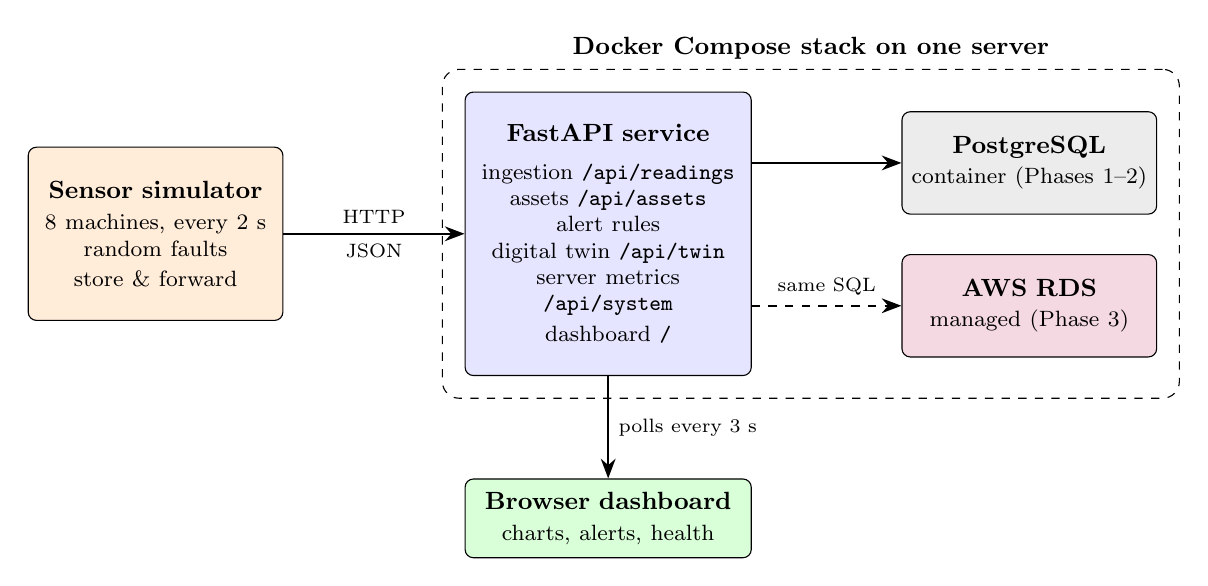
\begin{tikzpicture}[node distance=0.7cm and 1.1cm]
  \node[box=orange!15, text width=3.0cm, minimum height=2.2cm] (sim)
    {\textbf{Sensor simulator}\\[2pt]\footnotesize 8 machines, every 2 s\\ random faults\\ store \& forward};
  \node[box=blue!10, right=2.3cm of sim, text width=3.4cm, minimum height=3.6cm] (api)
    {\textbf{FastAPI service}\\[4pt]\footnotesize
     ingestion \texttt{/api/readings}\\ assets \texttt{/api/assets}\\ alert rules\\ digital twin \texttt{/api/twin}\\ server metrics \texttt{/api/system}\\ dashboard \texttt{/}};
  \node[box=gray!15, right=1.9cm of api, text width=3.0cm, minimum height=1.3cm, yshift=0.9cm] (pg)
    {\textbf{PostgreSQL}\\\footnotesize container (Phases 1--2)};
  \node[box=purple!15, below=0.5cm of pg, text width=3.0cm, minimum height=1.3cm] (rds)
    {\textbf{AWS RDS}\\\footnotesize managed (Phase 3)};
  \node[box=green!15, below=1.3cm of api, text width=3.4cm] (ui) {\textbf{Browser dashboard}\\\footnotesize charts, alerts, health};
  \draw[arr] (sim) -- node[above, font=\scriptsize]{HTTP} node[below, font=\scriptsize]{JSON} (api);
  \draw[arr] (api.east |- pg.west) -- (pg.west);
  \draw[arr, dashed] (api.east |- rds.west) -- node[above, font=\scriptsize, pos=0.5]{same SQL} (rds.west);
  \draw[arr] (api) -- node[right, font=\scriptsize]{polls every 3 s} (ui);
  \begin{scope}[on background layer]
    \node[layer, fit=(api)(pg)(rds), label={[font=\small\bfseries]above:Docker Compose stack on one server}] {};
  \end{scope}
\end{tikzpicture}
\caption{Mini-Predix architecture. Only the database connection string changes between the PostgreSQL container and RDS.}
\end{figure}

\subsection{Components}
\textbf{Simulator.} Each virtual machine produces temperature, vibration, RPM and pressure values that
drift around a normal operating point. Faults (overheating, bearing wear, overspeed, pressure leak)
start at random and ramp up over a few minutes, for example +12\,\textdegree{} C per minute for overheating.
If the API cannot be reached, batches are buffered and sent later, like Predix Machine's
store-and-forward feature. It uses only the Python standard library.

\textbf{Alert rules.} Every incoming reading is checked against a warning and a critical limit:
\begin{center}
\begin{tabular}{lccc}
\toprule
\textbf{Metric} & \textbf{Warning} & \textbf{Critical} & \textbf{Unit} \\
\midrule
Temperature & 90 & 105 & \textdegree{} C \\
Vibration & 7 & 10 & mm/s \\
RPM & 3700 & 3900 & rpm \\
Pressure & 28 & 32 & bar \\
\bottomrule
\end{tabular}
\end{center}

\textbf{Digital twin.} For each asset the API looks at the last 30 readings and computes a health score
(0--100) from how close each metric runs to its limits, the temperature trend in \textdegree{} C per minute
(least-squares slope), and, if the temperature is rising, a rough ``minutes until critical''
prediction. The dashboard shows this as \emph{healthy}, \emph{degraded} or \emph{critical}.

\textbf{Dashboard.} A single web page (Chart.js) shows fleet health cards, sensor history charts with
the warning and critical lines, recent alerts, and live server statistics.

\textbf{Quality.} Eight unit tests cover the alert rules and the digital-twin maths. The API reports its
own processing time in an \texttt{X-Process-Time-Ms} header so that we can separate server time from
network time in the benchmarks.

\subsection{Technology stack}
\begin{center}
\begin{tabularx}{\linewidth}{@{}p{4cm}L@{}}
\toprule
\textbf{Part} & \textbf{Technology} \\
\midrule
API and dashboard & Python 3.12, FastAPI, Uvicorn (2 workers), psycopg 3 connection pool, Chart.js \\
Database & PostgreSQL 16 container; AWS RDS PostgreSQL 18 (Phase 3) \\
Packaging & Docker images, Docker Compose \\
Deployment & \texttt{deploy/deploy\_vps.sh} (git archive + SSH), \texttt{deploy/use\_rds.sh} \\
Load testing & Own async benchmark script (Python, httpx), Matplotlib graphs \\
Version control & GitHub, small commits throughout the project \\
\bottomrule
\end{tabularx}
\end{center}

%================ MIGRATION ================
\section{Migration: What We Actually Did}
\subsection{Phase 1: Local (``on-premises'') baseline}
The whole stack is defined once in \texttt{docker-compose.yml}: a PostgreSQL container, the API container
and the simulator container. The same file runs on a laptop with Docker and, unchanged, on every
server below. This plays the role of GE's own data centers.

\subsection{Phase 2: Lift-and-shift to virtual machines}
\texttt{deploy/deploy\_vps.sh} copies the committed code to a server over SSH, creates a \texttt{.env} file with
a random database password, and starts the Compose stack. No application code changed between servers.

\begin{center}
\begin{tabularx}{\linewidth}{@{}p{3.6cm}p{2.3cm}p{3.6cm}L@{}}
\toprule
\textbf{Deployment} & \textbf{Location} & \textbf{Machine} & \textbf{Deploy time and extra setup} \\
\midrule
Mumbai VPS (Hostinger) & Mumbai & 4 vCPU, 16 GB RAM & 37 s; Docker already installed \\
Africa VPS & Africa & 3 vCPU, 4 GB RAM & 89 s; Docker already installed \\
AWS EC2 t3.micro & Mumbai (ap-south-1b) & 2 vCPU, 1 GB RAM & 68 s, after installing Docker and adding 2 GB swap by hand \\
AWS EC2 t3.medium & Mumbai (ap-south-1b) & 2 vCPU, 4 GB RAM & 73 s, after installing Docker; launched only for a same-size comparison and then terminated \\
\bottomrule
\end{tabularx}
\end{center}

On AWS we created the servers in the console: imported our SSH public key, chose Ubuntu, and created a
security group that opens only SSH (22) and the dashboard port (8090).

\subsection{Phase 3: Refactor to a managed database (AWS RDS)}
We created an RDS PostgreSQL \texttt{db.t4g.micro} instance (free-tier ``Sandbox'' template, single AZ,
20 GB storage, automatic daily backups) in the same availability zone as the EC2 server. Using the
console's ``Connect to an EC2 compute resource'' option, AWS created security groups so that
\textbf{only the EC2 server can reach the database}; it has no public address. The master password was
generated by AWS and stored only on the server, in a file readable by its owner.

The switch itself is one script, \texttt{deploy/use\_rds.sh}: it writes the RDS connection string into
\texttt{.env}, stops the PostgreSQL container and restarts the API with a small Compose override
(\texttt{docker-compose.rds.yml}). It took \textbf{40 seconds}, and the API created its tables in RDS on
start-up. The RDS instance itself took several minutes for AWS to provision.

\begin{figure}[H]
\centering
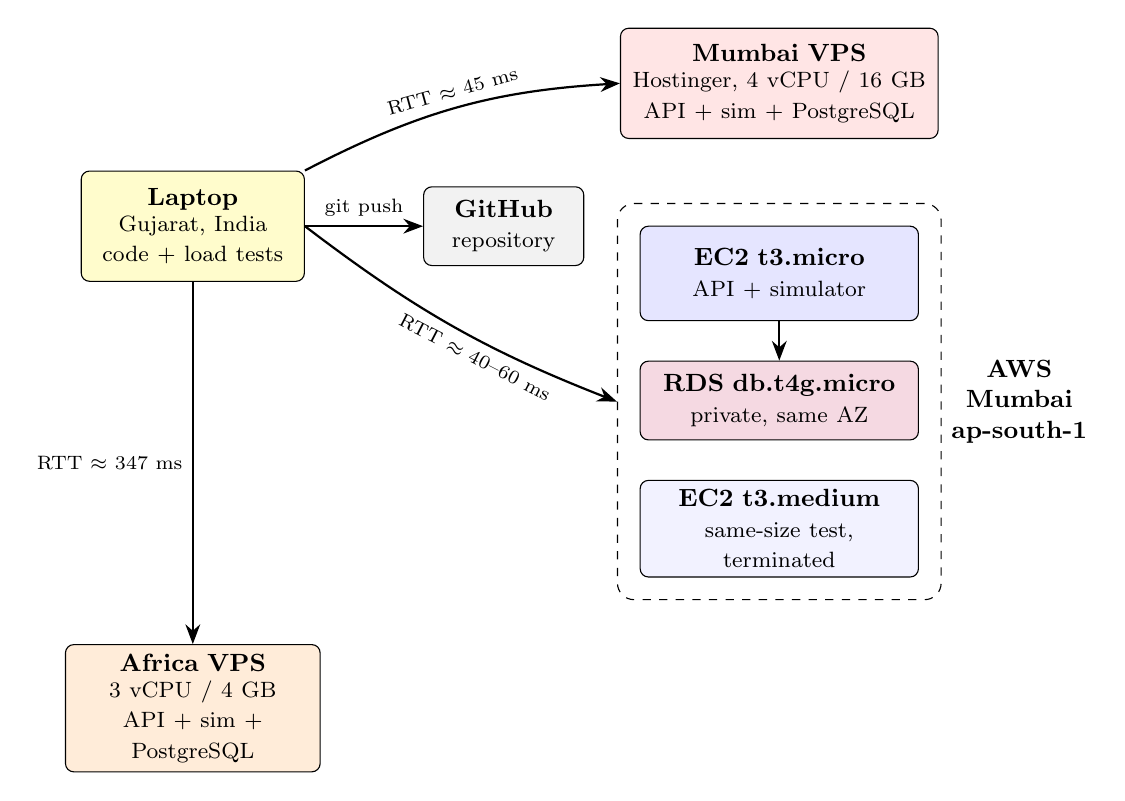
\begin{tikzpicture}[node distance=0.6cm and 0.8cm, every node/.style={font=\small}]
  \node[box=yellow!20, text width=2.6cm, minimum height=1.4cm] (lap) {\textbf{Laptop}\\\footnotesize Gujarat, India\\ code + load tests};
  \node[box=gray!10, right=1.5cm of lap, text width=1.8cm] (gh) {\textbf{GitHub}\\\footnotesize repository};
  % Mumbai VPS
  \node[box=red!10, above right=0.4cm and 4.0cm of lap, text width=3.8cm, minimum height=1.4cm] (mvps)
    {\textbf{Mumbai VPS}\\\footnotesize Hostinger, 4 vCPU / 16 GB\\ API + sim + PostgreSQL};
  % AWS region
  \node[box=blue!10, below=1.1cm of mvps, text width=3.3cm, minimum height=1.2cm] (ec2)
    {\textbf{EC2 t3.micro}\\\footnotesize API + simulator};
  \node[box=purple!15, below=0.5cm of ec2, text width=3.3cm, minimum height=1.0cm] (rds)
    {\textbf{RDS db.t4g.micro}\\\footnotesize private, same AZ};
  \node[box=blue!5, below=0.5cm of rds, text width=3.3cm, minimum height=1.0cm] (med)
    {\textbf{EC2 t3.medium}\\\footnotesize same-size test, terminated};
  \draw[arr] (ec2) -- (rds);
  \draw[arr] (lap) -- node[above, font=\scriptsize]{git push} (gh);
  % Africa
  \node[box=orange!15, below=4.6cm of lap, text width=3.0cm, minimum height=1.4cm] (afr)
    {\textbf{Africa VPS}\\\footnotesize 3 vCPU / 4 GB\\ API + sim + PostgreSQL};
  \begin{scope}[on background layer]
    \node[layer, fit=(ec2)(rds)(med), label={[font=\small\bfseries,align=center]right:AWS\\ Mumbai\\ ap-south-1}] (aws) {};
  \end{scope}
  \draw[arr] (lap.north east) to[bend left=12] node[above, font=\scriptsize, sloped]{RTT $\approx$ 45 ms} (mvps.west);
  \draw[arr] (lap.east) to[bend right=8] node[below, font=\scriptsize, sloped, pos=0.6]{RTT $\approx$ 40--60 ms} (aws.west);
  \draw[arr] (lap.south) -- node[left, font=\scriptsize, align=right]{RTT $\approx$ 347 ms} (afr.north);
\end{tikzpicture}
\caption{Deployments used in the project and the measured network round-trip time from the laptop.}
\end{figure}

\subsection{Problems found during migration}
\begin{itemize}
  \item \textbf{Start-up race.} On the first VPS deployment both API workers tried to create the tables at
        the same moment and one crashed. We fixed it with a PostgreSQL advisory lock around schema
        creation.
  \item \textbf{Small instance memory.} The t3.micro has 1 GB of RAM, so we added 2 GB of swap before
        running the database and API on it.
  \item \textbf{Shared server load.} The Mumbai VPS also runs other services (Grafana, Prometheus, test
        clients). Our on-server load test raised its load average to 7.65 on 4 CPUs, which slowed those
        services while the test ran (Section~12).
\end{itemize}

%================ METHOD ================
\section{Benchmark Method}
\texttt{benchmark/benchmark.py} runs \textbf{1, 5, 10, 25, 50 and 100 concurrent virtual users} for
\textbf{20 seconds per level}. Each user repeats requests in a loop with a realistic mix:
\begin{itemize}
  \item 30\% writes: a batch of 6 sensor readings (like edge gateways);
  \item 70\% reads: fleet health, latest readings and alerts (like dashboards).
\end{itemize}
It records throughput (successful requests per second), latency percentiles (p50, p95, p99) and
errors. Every 2 seconds it also samples the server's CPU, load average and memory through
\texttt{/api/system}.

We tested from two places:
\begin{itemize}
  \item \textbf{On the server} (``on-server''): the load generator runs on the same machine, so the
        network is removed and we measure \emph{server capacity}. The generator shares the CPU with the
        app; this affects every server in the same way.
  \item \textbf{From a laptop} in Gujarat over the internet: what a real user in India would feel.
        Laptop tests went up to 50 users.
\end{itemize}
Tests on the same server were never run at the same time. One laptop session had an unstable
connection (round-trip time jumping from about 80 to 370 ms) and one run overlapped with an on-server
test; those results were discarded and the tests repeated.

%================ RESULTS ================
\section{Performance Results}
\subsection{Server capacity (on-server tests)}
\begin{center}
\begin{tabularx}{\linewidth}{@{}Lcccc@{}}
\toprule
\textbf{Deployment} & \textbf{Peak req/s} & \textbf{p50 (5 users)} & \textbf{p95 (5 users)} & \textbf{CPU (5 users)} \\
\midrule
Mumbai VPS, 4 vCPU / 16 GB & \textbf{379.3} & 12.2 ms & 25.0 ms & 73\% \\
AWS t3.micro + RDS & 266.4 & 18.0 ms & 33.7 ms & 67\% \\
Africa VPS, 3 vCPU / 4 GB & 193.2 & 24.3 ms & 45.0 ms & 81\% \\
AWS t3.medium, 2 vCPU / 4 GB & 183.8 & 22.9 ms & 59.7 ms & 89\% \\
AWS t3.micro, 2 vCPU / 1 GB & 113.2 & 19.2 ms & 158.9 ms & 92\% \\
\bottomrule
\end{tabularx}
\end{center}
All deployments reached their peak throughput at 5 users. \textbf{No request failed in any test.}
Beyond the peak, requests queue up: at 100 users the p95 latency was 1.8 s on the Mumbai VPS and
3.2--4.5 s on the smaller machines.

\begin{figure}[H]
\centering
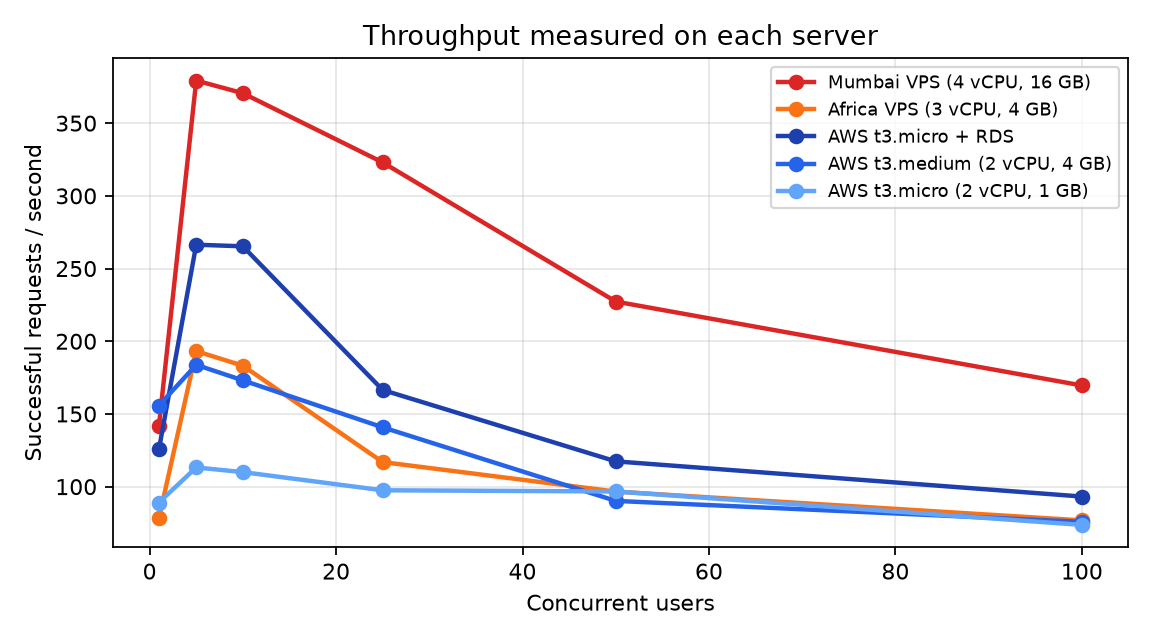
\includegraphics[width=0.92\linewidth]{onserver_throughput.png}
\caption{Throughput measured on each server.}
\end{figure}

\begin{figure}[H]
\centering
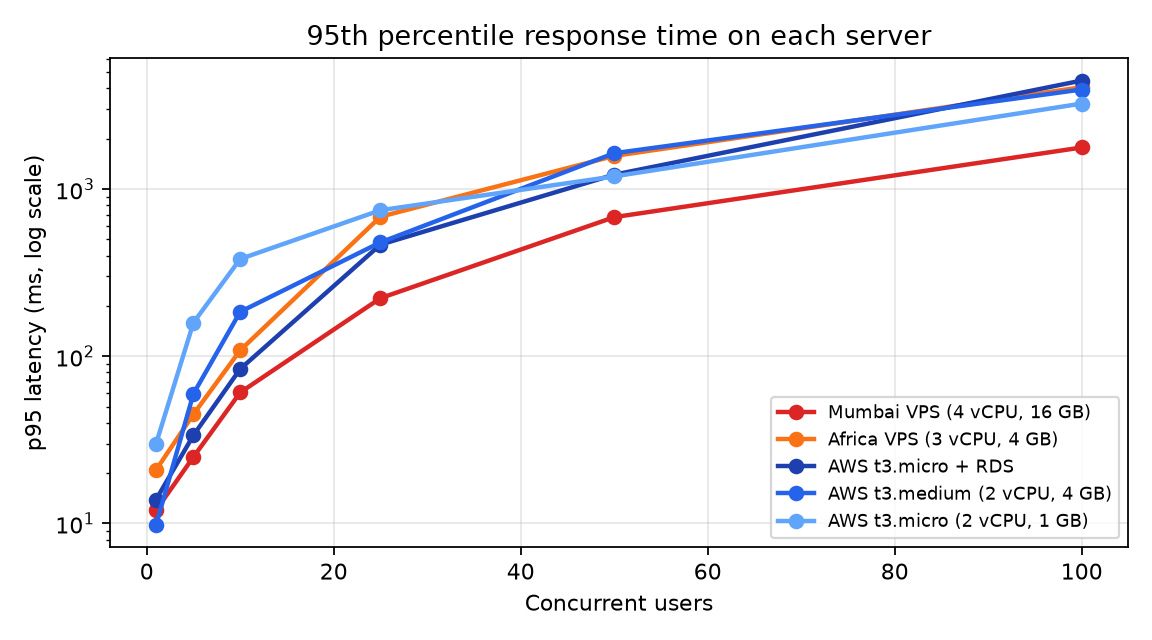
\includegraphics[width=0.92\linewidth]{onserver_latency_p95.png}
\caption{95th percentile latency measured on each server (log scale).}
\end{figure}

\subsection{What users feel (tests from the laptop)}
\begin{center}
\begin{tabularx}{\linewidth}{@{}Lccc@{}}
\toprule
\textbf{Deployment} & \textbf{Network RTT} & \textbf{p50 (1 user)} & \textbf{p50 (10 users)} \\
\midrule
AWS t3.micro + RDS (Mumbai) & 40.5 ms & 48.3 ms & 61.4 ms \\
AWS t3.medium (Mumbai) & 55.7 ms & 50.5 ms & 68.4 ms \\
AWS t3.micro (Mumbai) & 59.8 ms & 63.6 ms & 79.9 ms \\
Mumbai VPS & 44.6 ms & 73.1 ms & 76.2 ms \\
Africa VPS & \textbf{347.0 ms} & 364.4 ms & 368.9 ms \\
\bottomrule
\end{tabularx}
\end{center}

\begin{figure}[H]
\centering
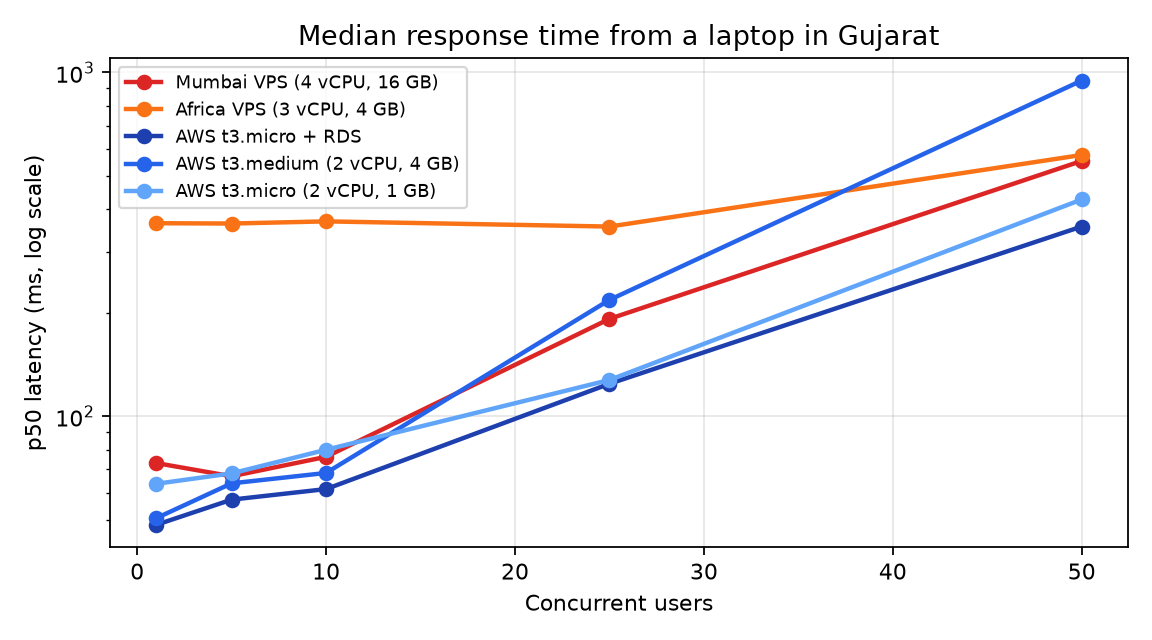
\includegraphics[width=0.92\linewidth]{internet_latency_p50.png}
\caption{Median latency seen from the laptop (log scale).}
\end{figure}

\subsection{Findings}
\begin{enumerate}
  \item \textbf{Same size means about the same speed.} The 4 GB Africa VPS (193 req/s) and the 4 GB AWS
        t3.medium (184 req/s) performed almost the same. AWS is not faster by itself.
  \item \textbf{A managed database is the biggest win for a small server.} Moving PostgreSQL off the
        1 GB t3.micro onto RDS raised throughput from 113 to 266 req/s (2.4$\times$) and cut p95 latency
        at 5 users from 159 ms to 34 ms, because the database no longer competes for the VM's CPU and
        memory. This is the effect GE was after when it moved to managed cloud services.
  \item \textbf{Location matters more than hardware for users.} The Africa server is about 7$\times$
        further away in network time than the Mumbai servers. For users in India a server in India wins,
        however powerful the distant one is.
  \item \textbf{Over the internet, network time dominates.} The server needs only about 5--25 ms per
        request, but a user in Gujarat sees 50--80 ms on a Mumbai server.
\end{enumerate}

%================ COST ================
\section{Cost Analysis}
\subsection{Prices used}
AWS prices are on-demand prices for Asia Pacific (Mumbai), Linux, from the AWS public price list
[10], with 1 month = 730 hours. VPS prices are what our team pays. We use 1 USD = Rs 96.5.

\begin{center}
\begin{tabularx}{\linewidth}{@{}Lr@{}}
\toprule
\textbf{Item} & \textbf{Price} \\
\midrule
EC2 t3.micro / t3.medium / t3.large / m6a.xlarge & \$0.0112 / 0.0448 / 0.0896 / 0.1111 per hour \\
RDS PostgreSQL db.t4g.micro / medium / large (single AZ) & \$0.021 / 0.084 / 0.167 per hour \\
EBS gp3 disk / RDS storage & \$0.0912 / \$0.131 per GB-month \\
Internet traffic out (after 100 GB free) & \$0.1093 per GB \\
Application Load Balancer & \$0.0239 per hour + \$0.008 per LCU-hour \\
Mumbai VPS (Hostinger), 4 vCPU / 16 GB & Rs 2,399 per month \\
Africa VPS, 3 vCPU / 4 GB & Rs 1,700 per month \\
Africa VPS, 4 vCPU / 8 GB & Rs 14,000 per 3 months (Rs 4,667 per month) \\
\bottomrule
\end{tabularx}
\end{center}
AWS figures below include 200 GB per month of internet traffic (\$10.93, about Rs 1,055), which AWS
charges for and our VPS plans include.

\subsection{Cost of each tested deployment}
\begin{center}
\begin{tabularx}{\linewidth}{@{}Lrrr@{}}
\toprule
\textbf{Deployment} & \textbf{Per month} & \textbf{Peak req/s} & \textbf{Per 100 req/s} \\
\midrule
Mumbai VPS, 4 vCPU / 16 GB & Rs 2,399 & 379.3 & \textbf{Rs 632} \\
Africa VPS, 3 vCPU / 4 GB & Rs 1,700 & 193.2 & Rs 880 \\
AWS t3.micro + RDS db.t4g.micro & Rs 3,752 & 266.4 & Rs 1,408 \\
AWS t3.micro + PostgreSQL container & Rs 2,020 & 113.2 & Rs 1,784 \\
AWS t3.medium + PostgreSQL container & Rs 4,387 & 183.8 & Rs 2,387 \\
\bottomrule
\end{tabularx}
\end{center}

\begin{figure}[H]
\centering
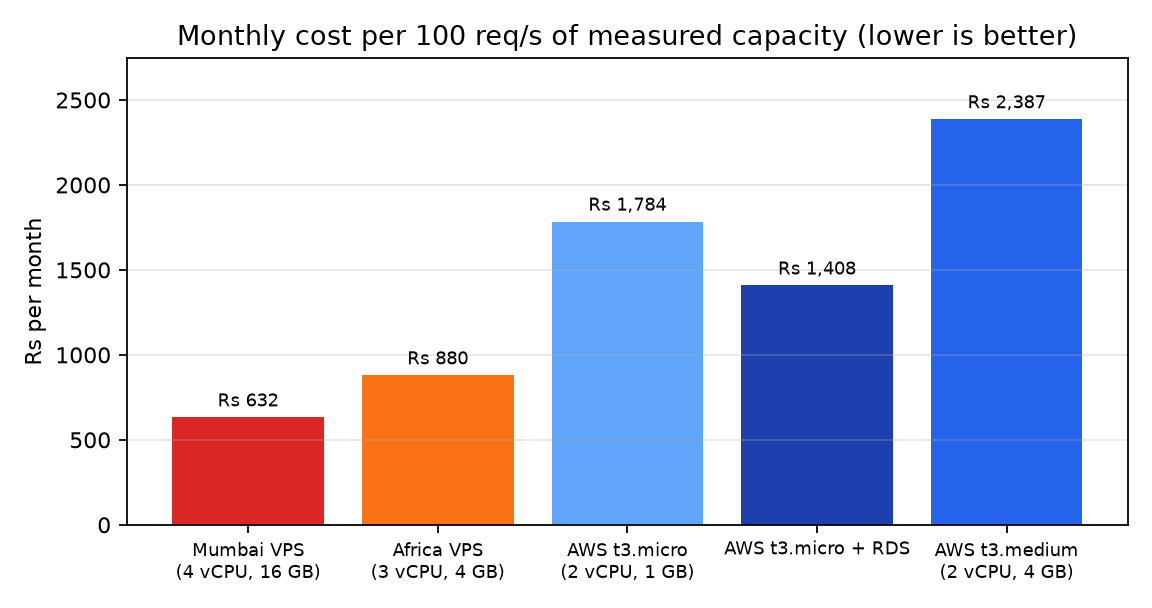
\includegraphics[width=0.92\linewidth]{cost_per_capacity.png}
\caption{Monthly cost for every 100 requests/second of measured capacity.}
\end{figure}

\subsection{A same-size machine on AWS}
\begin{center}
\begin{tabularx}{\linewidth}{@{}p{2.6cm}rp{3.2cm}rrr@{}}
\toprule
\textbf{Our VPS} & \textbf{VPS} & \textbf{AWS same size} & \textbf{On-demand} & \textbf{3-yr reserved} & \textbf{+ RDS} \\
\midrule
Africa 4 GB & Rs 1,700 & t3.medium & Rs 4,844 & Rs 2,849 & Rs 10,936 \\
Africa 8 GB & Rs 4,667 & t3.large & Rs 9,496 & Rs 5,503 & Rs 19,939 \\
Mumbai 16 GB & Rs 2,399 & m6a.xlarge & Rs 10,580 & Rs 5,852 & Rs 21,454 \\
\bottomrule
\end{tabularx}
\end{center}
The AWS columns include a disk the same size as the VPS disk. ``+ RDS'' adds a managed database
(db.t4g.medium or db.t4g.large with 50 GB). Over 3 years the 16 GB server costs \textbf{Rs 86,364 on
the VPS}, against Rs 2.1 lakh (3-year reserved) to Rs 3.8 lakh (on-demand) on AWS, or Rs 7.7 lakh with
a managed database.

\begin{figure}[H]
\centering
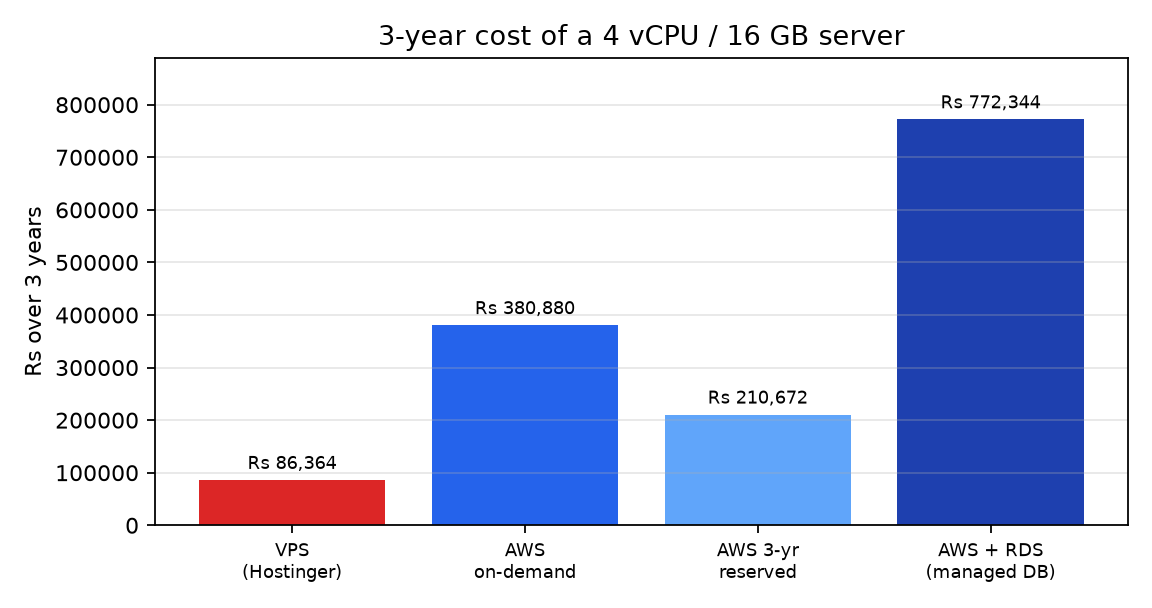
\includegraphics[width=0.85\linewidth]{tco_3yr.png}
\caption{3-year cost of a 4 vCPU / 16 GB server.}
\end{figure}

\subsection{Scaling scenario: a daily 10$\times$ traffic spike}
We modelled a load of 200 req/s that rises to 2,000 req/s for 4 hours every day, like a cricket match
or a Tatkal booking window. Capacities come from our measurements: 379 req/s per Mumbai VPS and
184 req/s per t3.medium.

\begin{center}
\begin{tabularx}{\linewidth}{@{}p{3.4cm}Lr@{}}
\toprule
\textbf{Option} & \textbf{How it handles the peak} & \textbf{Per month} \\
\midrule
Mumbai VPS fleet & 6 servers sized for the peak, running all month, set up by hand & Rs 14,394 \\
AWS Auto Scaling & 2 t3.medium always on, up to 11 during the spike, plus a load balancer & Rs 24,975 \\
\bottomrule
\end{tabularx}
\end{center}
Even with spiky traffic the VPS fleet is cheaper on paper, mainly because AWS charges for internet
traffic (about 40\% of the AWS bill here) and our VPS is unusually cheap for its size. The next
section shows what that lower price leaves out.

\begin{figure}[H]
\centering
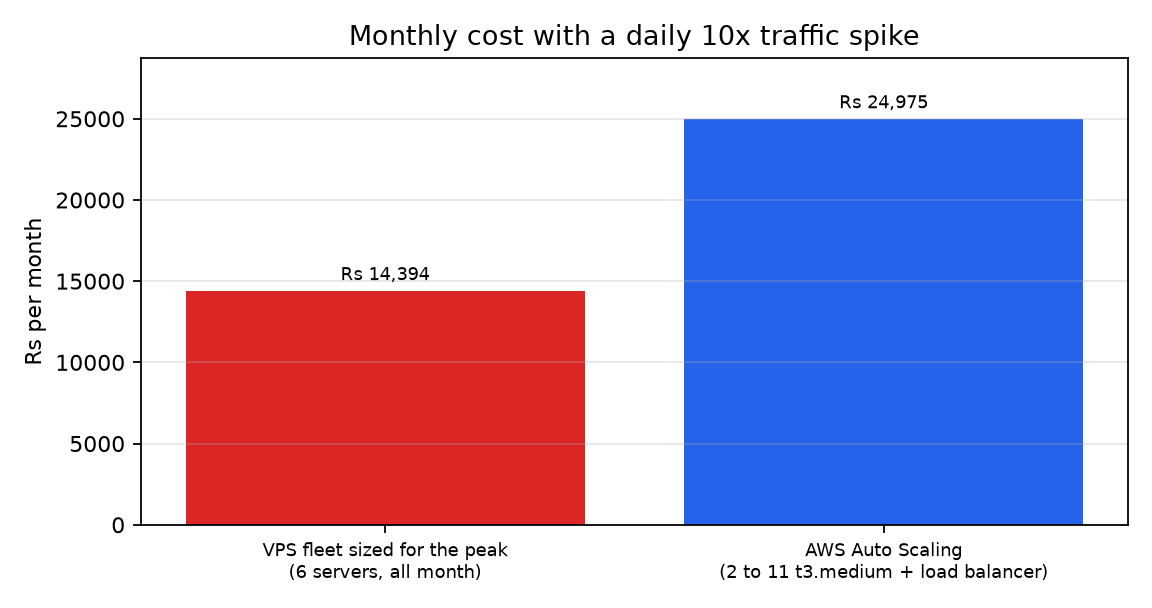
\includegraphics[width=0.85\linewidth]{spike_scenario.png}
\caption{Monthly cost with a daily 10$\times$ traffic spike.}
\end{figure}

%================ OPS ================
\section{Operations and Scaling Effort}
The VPS wins on price because it is a \textbf{bare machine}: we get CPU, RAM and a disk, and everything
else is our job. This section lists what that meant in practice during this project.

\subsection{What we had to do ourselves}
\begin{center}
\begin{tabularx}{\linewidth}{@{}p{3.1cm}LL@{}}
\toprule
\textbf{Task} & \textbf{VPS (what we did)} & \textbf{AWS (what we did)} \\
\midrule
Get a server & Already rented; a new one means ordering a plan from the provider & Launched from the console in about 1 minute \\
Install Docker, swap, ports & By hand over SSH & Same by hand on EC2 (EC2 is still IaaS) \\
Firewall & The Mumbai VPS had no firewall rules (INPUT policy ACCEPT); we would have to set this up & Security group created in the launch wizard; RDS reachable only from EC2 \\
Database setup & PostgreSQL container, password generated by our script & RDS created in the console, password generated by AWS \\
Backups & \textbf{None.} We would have to write, schedule and test them & RDS automatic daily backups, on by default \\
Database failover & Not possible on one VPS & One option (Multi-AZ) in RDS \\
Monitoring & Only our own \texttt{/api/system} endpoint & RDS Database Insights (7 days free) plus our endpoint \\
Moving the DB off the app server & Needs a second server, network setup and a data copy & 40-second switch with \texttt{deploy/use\_rds.sh} \\
\bottomrule
\end{tabularx}
\end{center}

\subsection{A problem we actually hit: noisy neighbours}
The Mumbai VPS also runs Grafana, Prometheus, Langfuse and test clients. During our on-server load
test its load average rose to \textbf{7.65 on 4 CPUs}, slowing every other service on the machine. On a
shared, self-managed server one application can starve the others. On AWS the database on RDS and each
EC2 instance have their own resources.

\subsection{How each option scales}
\begin{figure}[H]
\centering
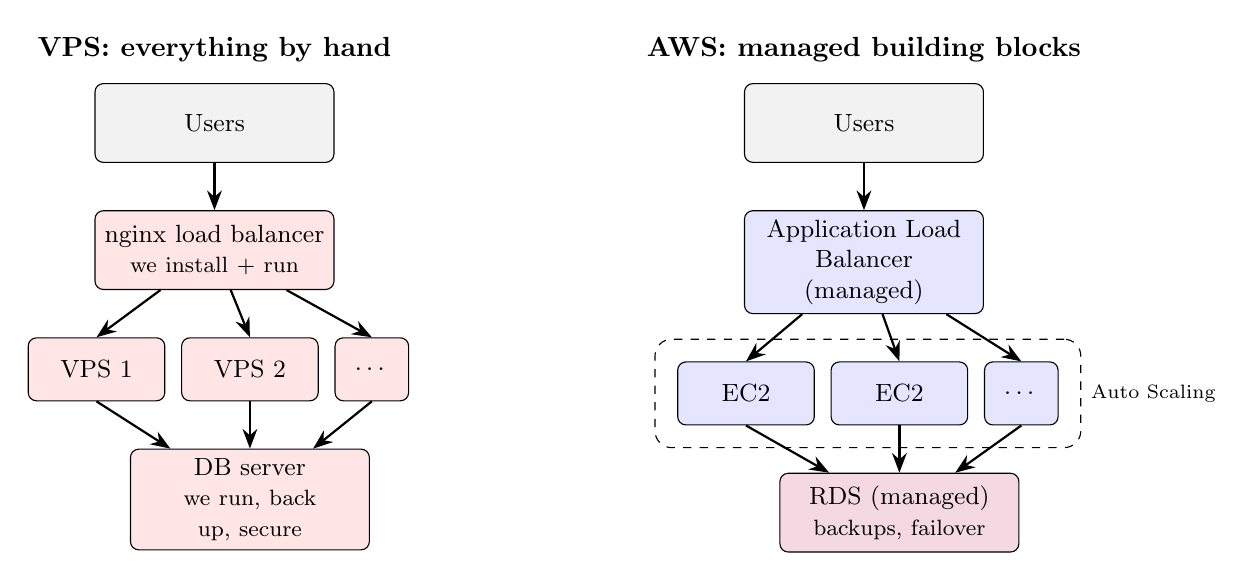
\begin{tikzpicture}[node distance=0.45cm and 0.5cm, every node/.style={font=\small}]
  % VPS side
  \node[box=gray!10, text width=2.8cm] (u1) {Users};
  \node[box=red!10, below=0.6cm of u1, text width=2.8cm] (lb1) {nginx load balancer\\\footnotesize we install + run};
  \node[box=red!10, below left=0.6cm and -0.9cm of lb1, text width=1.5cm, minimum height=0.8cm] (v1) {VPS 1};
  \node[box=red!10, right=0.2cm of v1, text width=1.5cm, minimum height=0.8cm] (v2) {VPS 2};
  \node[box=red!10, right=0.2cm of v2, text width=0.7cm, minimum height=0.8cm] (v3) {\dots};
  \node[box=red!10, below=0.6cm of v2, text width=2.8cm] (db1) {DB server\\\footnotesize we run, back up, secure};
  \draw[arr] (u1) -- (lb1);
  \foreach \n in {v1,v2,v3} { \draw[arr] (lb1) -- (\n.north); \draw[arr] (\n.south) -- (db1); }
  \node[above=0.15cm of u1, font=\bfseries] {VPS: everything by hand};
  % AWS side
  \node[box=gray!10, right=5.2cm of u1, text width=2.8cm] (u2) {Users};
  \node[box=blue!10, below=0.6cm of u2, text width=2.8cm] (lb2) {Application Load\\Balancer (managed)};
  \node[box=blue!10, below left=0.6cm and -0.9cm of lb2, text width=1.5cm, minimum height=0.8cm] (e1) {EC2};
  \node[box=blue!10, right=0.2cm of e1, text width=1.5cm, minimum height=0.8cm] (e2) {EC2};
  \node[box=blue!10, right=0.2cm of e2, text width=0.7cm, minimum height=0.8cm] (e3) {\dots};
  \node[box=purple!15, below=0.6cm of e2, text width=2.8cm] (db2) {RDS (managed)\\\footnotesize backups, failover};
  \draw[arr] (u2) -- (lb2);
  \foreach \n in {e1,e2,e3} { \draw[arr] (lb2) -- (\n.north); \draw[arr] (\n.south) -- (db2); }
  \begin{scope}[on background layer]
    \node[layer, fit=(e1)(e3), label={[font=\scriptsize]right:Auto Scaling}] {};
  \end{scope}
  \node[above=0.15cm of u2, font=\bfseries] {AWS: managed building blocks};
\end{tikzpicture}
\caption{Scaling out. On the VPS every box is a server we buy, set up and maintain. On AWS the load
balancer, scaling group and database are managed services.}
\end{figure}

\begin{center}
\begin{tabularx}{\linewidth}{@{}p{3.3cm}LL@{}}
\toprule
\textbf{To handle more traffic} & \textbf{VPS} & \textbf{AWS} \\
\midrule
Bigger machine (vertical) & Upgrade the plan, or rent a new server and migrate data by hand & Stop the instance, change the type, start it (a few minutes) \\
More machines (horizontal) & Rent N servers, install Docker on each, run a load balancer, point all of them at a shared database & Auto Scaling group behind a load balancer adds and removes servers automatically \\
Shared database & Run and secure a separate database server ourselves & RDS endpoint reachable by all instances; scale with one setting or add read replicas \\
Scale down after a spike & Monthly or quarterly plans, so we keep paying for the peak & Instances terminate and billing stops per second \\
A server dies & Restore by hand; nothing restarts it & Auto Scaling replaces it; RDS fails over (Multi-AZ) \\
\bottomrule
\end{tabularx}
\end{center}

In the spike scenario the VPS fleet is cheaper on paper (Rs 14,394 against Rs 24,975), but it needs
\textbf{6 servers set up, patched and monitored by hand}, a load balancer we run ourselves and a shared
database, and it stays sized for the peak all month. AWS does the same job with no manual steps once
it is configured. Our own t3.medium comparison server ran for well under an hour and cost only a few rupees, because
AWS bills per second; a monthly VPS plan cannot do that.

\subsection{Where the hidden VPS cost comes from}
\begin{center}
\begin{tabularx}{\linewidth}{@{}p{4.6cm}LL@{}}
\toprule
\textbf{Hidden cost} & \textbf{VPS} & \textbf{AWS} \\
\midrule
Admin time (backups, updates, monitoring) & About 4 h/month assumed, about Rs 2,000 at Rs 500/h & Much lower with managed services \\
Risk of data loss & High until backups are built and tested & Low (automatic backups) \\
Downtime when hardware fails & Hours, until someone fixes it & Minutes (replacement or failover) \\
Time to add capacity for an event & Days (order, set up, test) & Minutes \\
\bottomrule
\end{tabularx}
\end{center}
The admin-time figure is an assumption, not a measurement, but at that rate the hidden cost of a
self-managed server is close to the price of a small RDS database.

\textbf{Summary.} The VPS is the cheapest way to \emph{run} Mini-Predix, but the hardest to
\emph{operate and grow}. AWS costs more per unit of capacity, and the difference pays for managed
backups, failover, isolation and automatic scaling.

%================ RECOMMENDATION ================
\section{Recommendation}
\begin{center}
\begin{tabularx}{\linewidth}{@{}p{4.6cm}p{3.6cm}L@{}}
\toprule
\textbf{Situation} & \textbf{Best choice} & \textbf{Why} \\
\midrule
Student project, demo, steady small load & \textbf{Mumbai VPS} & Cheapest by far, fast in India, enough capacity (379 req/s) \\
Users mainly in India & Mumbai (VPS or AWS) & About 45 ms against 347 ms from Africa \\
Data must never be lost, or downtime is costly & \textbf{AWS with RDS (Multi-AZ)} & Managed backups and failover \\
Traffic unpredictable or growing fast & \textbf{AWS} & Scale in minutes without buying servers in advance \\
Long-term steady production load & VPS, or AWS with a 3-year commitment & Commitments cut AWS cost by about 45\% \\
Best of both & \textbf{Hybrid} & Steady base on VPS, managed database or bursts on AWS \\
\bottomrule
\end{tabularx}
\end{center}

\subsection{Link back to the GE case}
GE moved to AWS less for raw price than for speed and less operational work: its plan to shrink from
34 data centers to 4 meant far less hardware and staff to manage [4]. Our results show the same
trade-off at small scale. Rented servers are cheaper per unit of capacity, which is why companies such
as Basecamp and Dropbox moved steady workloads back out of the public cloud [11,12]. What the cloud
really sells is managed services and elasticity. Predix also struggled partly because GE built and ran
its own cloud infrastructure instead of using a provider's [7,8]; GE later made Predix available on AWS and Azure [3].
The lesson for us is the same: use managed services where they remove real work, keep steady and
simple workloads on cheap infrastructure, and compare the bill honestly.

%================ CONCLUSION ================
\section{Conclusion}
GE's Predix shows both the promise and the difficulty of cloud transformation. The ideas behind it,
edge computing, time-series data and digital twins, became standard practice, and GE's own migration
to AWS reduced the work of running data centers. Building and selling its own general-purpose
industrial cloud, however, proved too costly.

Our Mini-Predix exercise reproduced this journey: the same Docker stack ran unchanged on a laptop setup,
two VPS servers and AWS EC2, and a 40-second change moved its database to AWS RDS. The measurements
show that:
\begin{itemize}
  \item same-size machines perform about the same on a VPS and on AWS (193 against 184 req/s);
  \item a managed database made a small AWS server 2.4$\times$ faster;
  \item location decides what users feel (45 ms Mumbai against 347 ms Africa);
  \item the VPS is about 4$\times$ cheaper for a steady load, while AWS costs more but brings scaling,
        backups, failover and much less manual work.
\end{itemize}
For a small, steady workload like ours a VPS in India is the best value. As soon as reliability,
growth or unpredictable traffic matter, the managed AWS services become worth their price, which is
the same reasoning that led GE to the cloud.

%================ REFERENCES ================
\section*{References}
\addcontentsline{toc}{section}{References}
\begin{enumerate}[label={[\arabic*]},leftmargin=2.2em,itemsep=4pt]
  \item GE Press Release, ``GE Announces Predix Cloud'', Aug 2015. \url{https://www.ge.com/news/press-releases/ge-announces-predix-cloud-worlds-first-cloud-service-built-industrial-data-and}
  \item Cloud Foundry Foundation, ``A Platform for the Internet of Very Important Things''. \url{https://www.cloudfoundry.org/blog/a-platform-for-the-internet-of-very-important-things/}
  \item Data Center Knowledge, ``GE Unveils Predix, Its Industrial Strength Cloud'', 2015. \url{https://www.datacenterknowledge.com/cloud/ge-unveils-predix-its-industrial-strength-cloud}
  \item Constellation Research, ``GE, Capital One Give AWS the Rub at re:Invent'', 2015. \url{https://www.constellationr.com/content/ge-capital-one-give-aws-rub-reinvent}
  \item Amazon Press, ``General Electric Names AWS Its Preferred Cloud Provider'', Oct 2017. \url{https://press.aboutamazon.com/2017/10/general-electric-names-aws-its-preferred-cloud-provider}
  \item GE Digital, ``Predix Platform for the Industrial Internet'' Datasheet. \url{https://www.ge.com/digital/sites/default/files/download_assets/Predix-Platform-for-the-Industrial-Internet-Datasheet.pdf}
  \item CIO Dive, ``Have GE's Digital Transformation Efforts Hit a Snag?'', 2017. \url{https://www.ciodive.com/news/have-ges-digital-transformation-efforts-hit-a-snag/503736/}
  \item CIO Dive, ``GE to Scale Back Predix amid Companywide Restructure'', 2017. \url{https://www.ciodive.com/news/ge-to-scale-back-predix-amid-companywide-restructure/510758/}
  \item POWER Magazine, ``GE Shelves Plans to Spin Off Digital Business'', 2019. \url{https://www.powermag.com/ge-shelves-plans-to-spin-off-digital-business/}
  \item AWS Price List API, Asia Pacific (Mumbai): EC2, RDS, EBS, data transfer and ELB offer files, retrieved Oct 2026. \url{https://pricing.us-east-1.amazonaws.com/offers/v1.0/aws/index.json}
  \item D. H. Hansson, ``Why we're leaving the cloud'', 37signals, 2022. \url{https://world.hey.com/dhh/why-we-re-leaving-the-cloud-654b47e0}
  \item Dropbox Tech Blog, ``Inside the Magic Pocket'', 2016. \url{https://dropbox.tech/infrastructure/inside-the-magic-pocket}
  \item Project repository (code, benchmark data, cost model): \url{https://github.com/paramsavjani/it457-mini-predix}
\end{enumerate}

\end{document}
